%!TEX options = -shell-escape

\documentclass[glossy]{beamer}

% Fonts
\usepackage[utf8]{inputenc}
\usepackage{lmodern}
\usepackage[T1]{fontenc}
\usepackage{soul}

% Beamer
\usetheme{DarkConsole}

\setbeamertemplate{navigation symbols}{}

% Tikz
\usepackage{tikz}
\usetikzlibrary{tikzmark, arrows, decorations, decorations.pathreplacing, positioning, shadows}
\tikzset{every picture/.style={font issue=\scriptsize},
         font issue/.style={execute at begin picture={#1\selectfont}}
}

  \tikzset{
  shadowed/.style={preaction={transform canvas={shift={(2pt,-1pt)}},draw=gray,very thick}},
}

\tikzstyle{callout}=[remember picture, ->, >=stealth, overlay, red, ultra thick, align=center, anchor=west, drop shadow={shadow xshift=.8cm,shadow yshift=-.8cm}]

\tikzstyle{codebox}=[rectangle, draw=black, very thick, minimum size=7mm]

% Colorv
\usepackage{color}
\definecolor{bg}{rgb}{0.1, 0.1, 0.1}

% Minted
\usepackage{minted}
\newminted{console}{autogobble, fontsize=\large, escapeinside=??}
\newmintinline{console}{autogobble, escapeinside=??}
\newmintedfile{console}{fontsize=\large, escapeinside=??, bgcolor=bg}
\newmintedfile{bash}{fontsize=\large, escapeinside=??, bgcolor=bg}
\newmintedfile{diff}{fontsize=\large, style=vim, bgcolor=bg}
\newmintedfile{text}{fontsize=\large, bgcolor=bg}
\newminted{vctreestatus}{autogobble, fontsize=\large, bgcolor=bg}
\usemintedstyle{trac}

% GraphicX
\usepackage{graphicx}
\graphicspath{{img/}}

% Macros
\newcommand{\refer}[1]{([shift={(.25em,.25em)}]pic cs:#1)}
\newcommand{\filename}[1]{\texttt{\textbf{\emph{#1}}}}

\usepackage[svgpath=img/]{svg}
\usepackage[linewidth=1pt]{mdframed}
\usepackage{csquotes}

% Meta
\title{Git Boot Camp}
\author{Jesse Talavera-Greenberg}
\date{}
\begin{document}

% Things to note:
% Provide a git config in advance
% Avoid using vi
% Don't screw around with the PATH

\begin{frame}[fragile=singleslide]
  \frametitle{Git Boot Camp}
  \framesubtitle{Jesse Talavera-Greenberg}
  \begin{figure}
    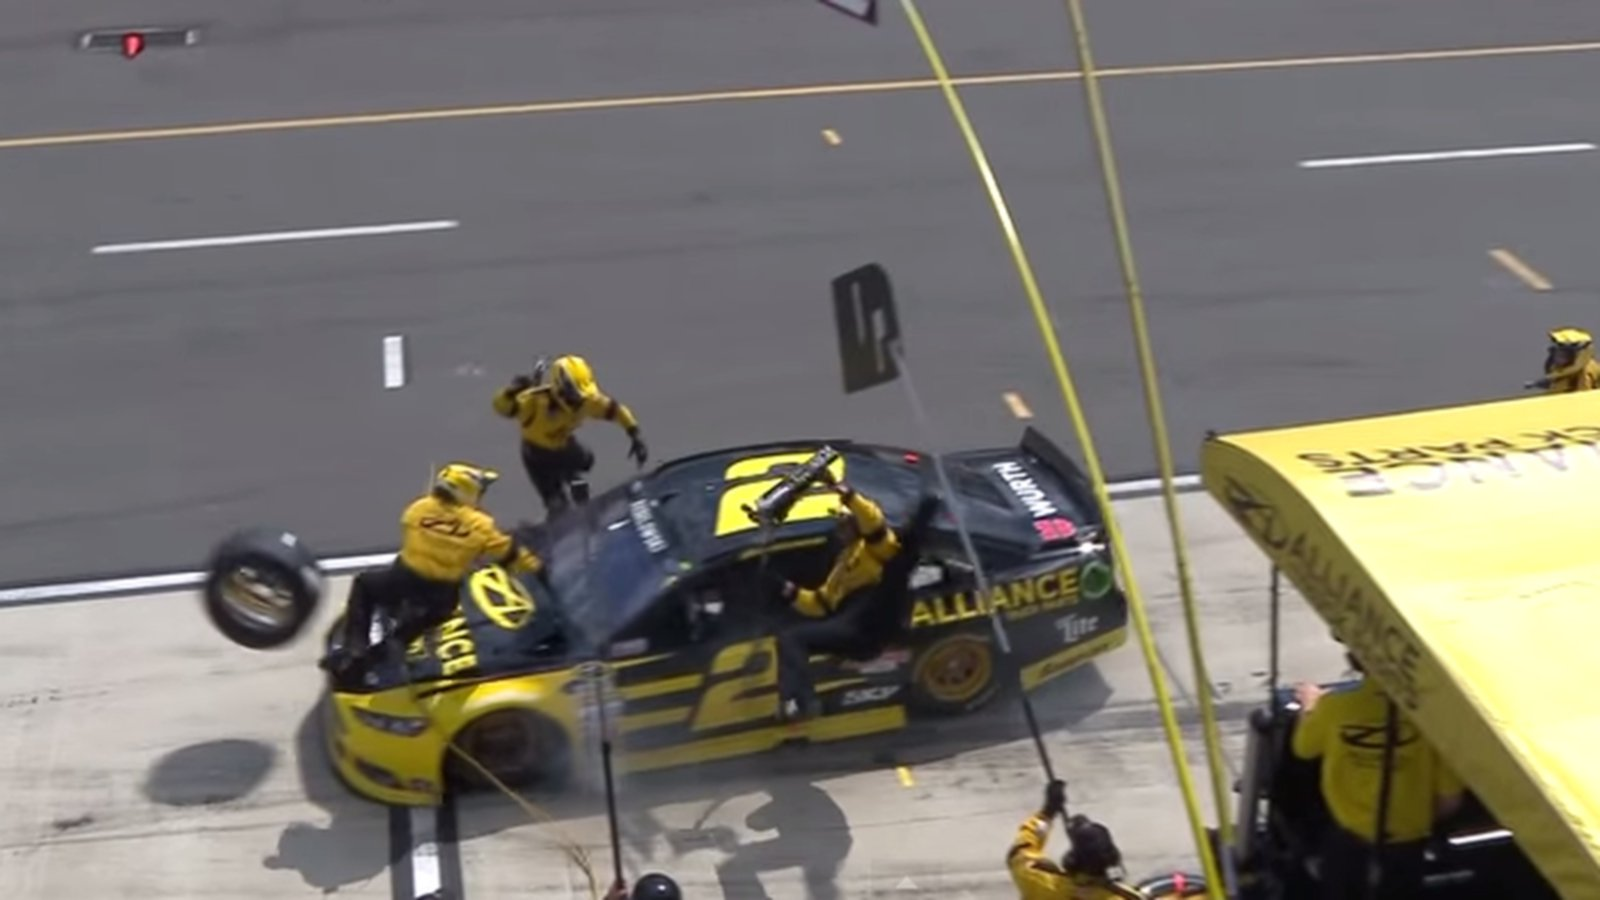
\includegraphics[width=.9\columnwidth]{nascar}
    \centering
  \end{figure}
  \begin{tikzpicture}[callout, line width=1mm]
    \draw (4cm, 6cm) node [anchor=south] (dont_git) {\large \textbf{People who don't use Git}} -> (3.8cm, 4cm);
    \draw (dont_git.south) -> (4.6cm, 4.7cm);
    \draw (dont_git.south) -> (6.4cm, 3.6cm);

    \draw (8cm, 2cm) node [anchor=north] {\large \textbf{The person who merges changes}} -> (5.5cm, 2.75cm);
    \draw (2.75cm, 1.5cm) node [anchor=north] {\large \textbf{The code you lost}} -> (2.5cm, 2.7cm);
  \end{tikzpicture}
\end{frame}

\begin{frame}[fragile=singleslide]
  \frametitle{Disclaimers}

  \begin{itemize}
    \item I am not the grader for this course.
    \item This boot camp is entirely voluntary.
    \item All opinions expressed are my own.
    \item Correctness is likely, but not guaranteed.
  \end{itemize}
\end{frame}

\begin{frame}[fragile=singleslide]
  \frametitle{Today}

  \begin{itemize}
    \item Version control
    \item Git fundamentals
    \item Collaboration workflows
    \begin{itemize}
      \item No, not Dropbox
    \end{itemize}
    \item Contributing to open source projects
    \item Issue tracking
  \end{itemize}
\end{frame}

\begin{frame}[fragile=singleslide]
  \frametitle{To Clarify}

  \begin{columns}[t]
    \begin{column}{6cm}
      \begin{figure}
        \centering
        \textbf{Git}
        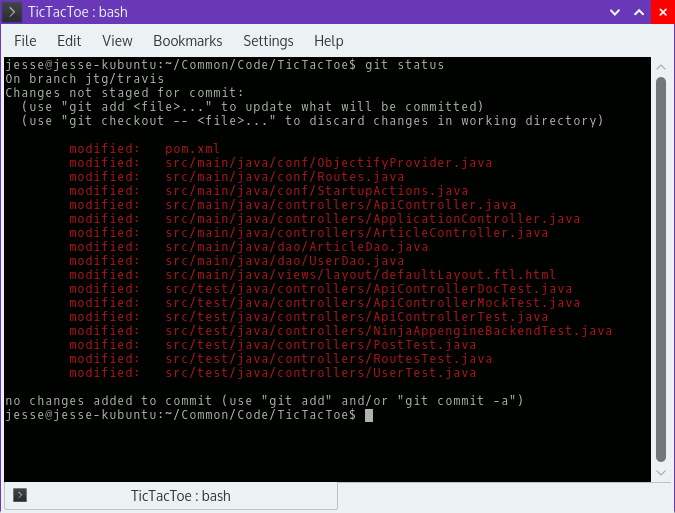
\includegraphics[width=.9\columnwidth]{git}
      \end{figure}
    \end{column}

    \begin{column}{6cm}
      \begin{figure}
        \centering
        \textbf{GitHub}
        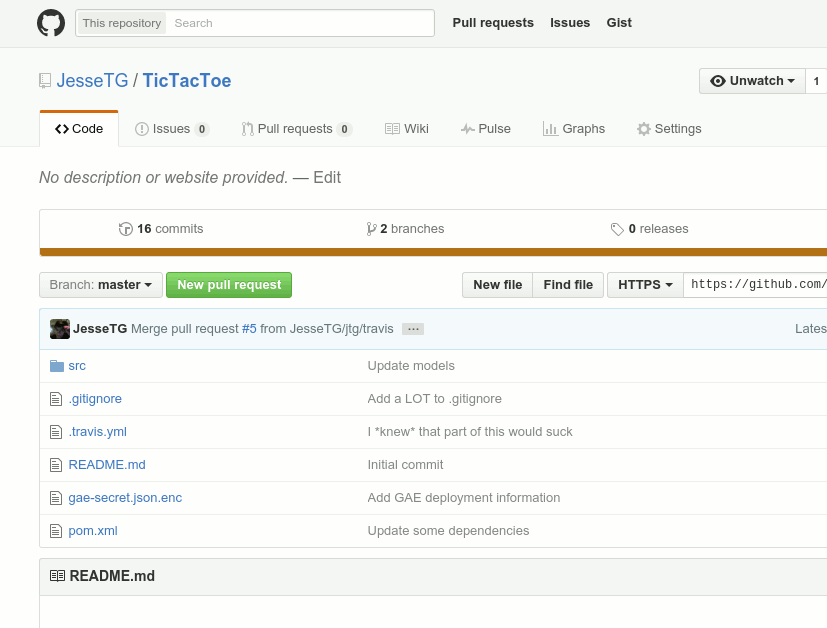
\includegraphics[width=.9\columnwidth]{github}
      \end{figure}
    \end{column}
  \end{columns}
  \hfill \break
  \textbf{Other Git-compatible code hosts:}
  \begin{itemize}
    \item BitBucket
    \item GitLab
    \item SourceForce
    \item Your own server
  \end{itemize}
\end{frame}

\begin{frame}[fragile=singleslide]
  \frametitle{Git Done Wrong}

  \begin{itemize}
    \item Write code
    \item Try GitHub or Bitbucket for a while
    \item Make a few giant-ass commits
    \item Get lots of merge conflicts when you try to pull your teammate's code
    \item Try to resolve these merge conflicts
    \item Clone the repo and start all over
    \item Do all of that two or three more times
    \item Give up and use Dropbox, e-mail, and/or Facebook
  \end{itemize}
\end{frame}

\begin{frame}[fragile=singleslide]
  \frametitle{\textcolor{red}{You will do better, or else.}}

  \begin{figure}
    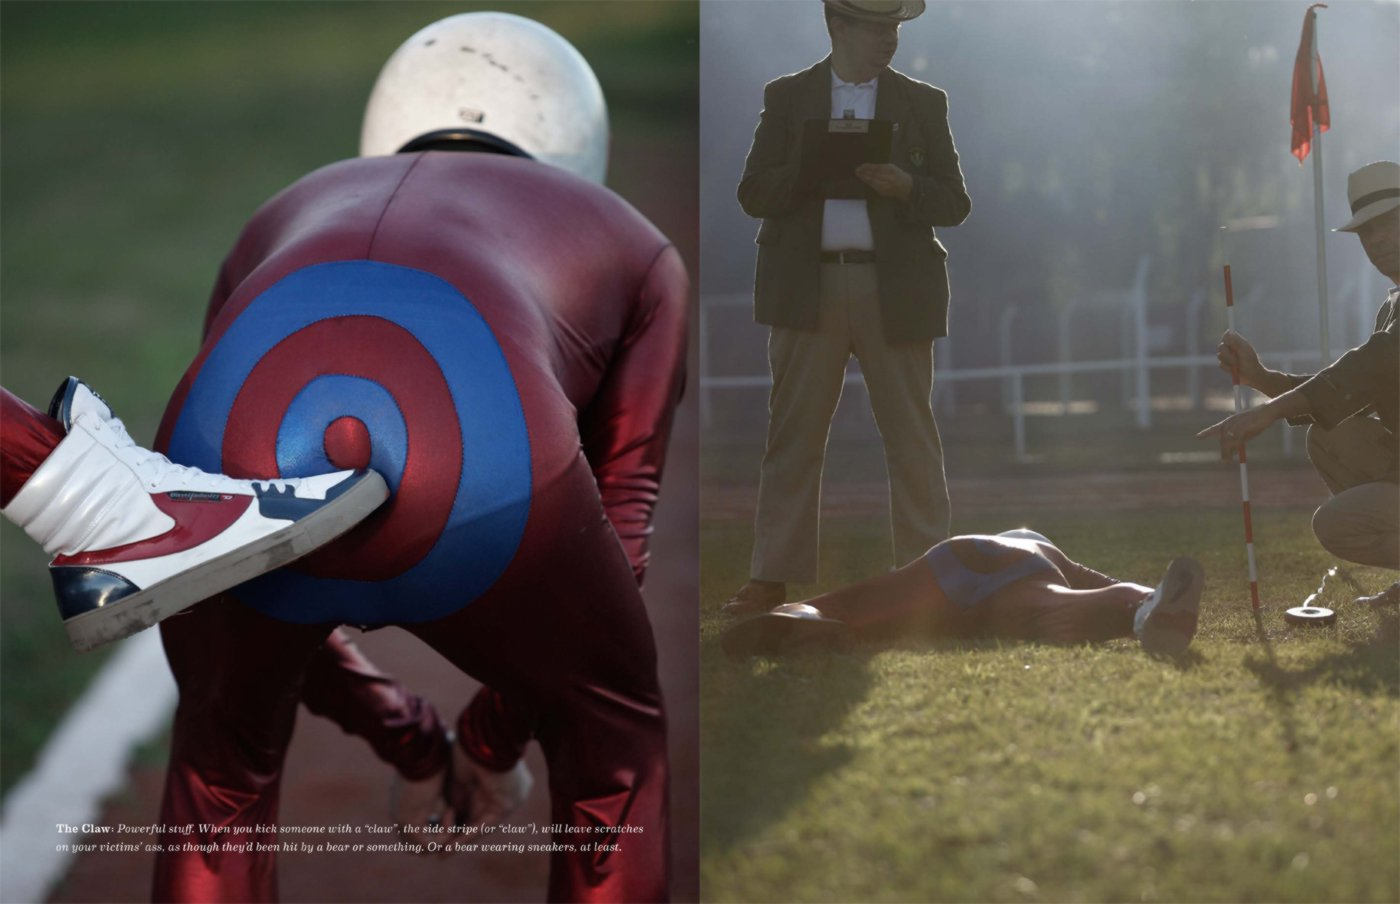
\includegraphics[width=.9\columnwidth]{whoopass}
    \centering
  \end{figure}
  \begin{tikzpicture}[callout, line width=2mm]
    \draw (2.25cm, 7cm) node [anchor=east] {\huge \textbf{You}} -> (3.5cm, 7cm);
    \draw (3.75cm, 2cm) node [anchor=north] {\huge \textbf{My foot}} -> (2.5cm, 3.5cm);
    \draw (9cm, 6cm) node [anchor=south] {\huge \textbf{You, elsewhere}} -> (8.5cm, 4cm);
  \end{tikzpicture}
\end{frame}

\begin{frame}[fragile=singleslide]
  \frametitle{Why version control?}

  \begin{itemize}
    \item See your code's entire history
    \item Make changes without destroying code
    \begin{itemize}
      \item Instantly scrap things that go wrong
      \item Work on different modules at once
    \end{itemize}
    \item Keep a good copy at all times
    \item No need to back up your work!
  \end{itemize}
\end{frame}

\begin{frame}[fragile=singleslide]
  \frametitle{Why version control?}

  \textcolor{green}{\enquote{Hey, where did the fix for that memory leak go?}}
  \begin{flushright}
    \textcolor{red}{\enquote{I did a thing with textures. Can't you put it back in?}}
  \end{flushright}
  \textcolor{green}{\enquote{I don't remember where the original bug was.}}
  \begin{flushright}
    \textcolor{red}{\enquote{Fuck.}}
  \end{flushright}

  \begin{columns}[b]
    \begin{column}{6cm}
      \begin{figure}
        \centering
        \includesvg[width=0.8\columnwidth]{coder}
      \end{figure}
    \end{column}

    \begin{column}{6cm}
      \begin{figure}
        \centering
        \includesvg[width=0.8\columnwidth]{angry-coder}
      \end{figure}
    \end{column}

  \end{columns}
\end{frame}

\begin{frame}[fragile=singleslide]
  \frametitle{Why version control?}

  \textcolor{green}{\enquote{Does Rob have the new JSON loader ready?  He's not online.}}
  \begin{flushright}
    \textcolor{red}{\enquote{I thought you gave it to him?}}
  \end{flushright}
  \textcolor{green}{\enquote{You told \emph{him} to write it!}}
  \begin{flushright}
    \textcolor{red}{\enquote{Wait, he just texted me...his cat peed on his laptop.}}
  \end{flushright}

  \begin{columns}[b]
    \begin{column}{6cm}
      \begin{figure}
        \centering
        \includesvg[width=0.8\columnwidth]{coder}
      \end{figure}
    \end{column}

    \begin{column}{6cm}
      \begin{figure}
        \centering
        \includesvg[width=0.8\columnwidth]{angry-coder}
      \end{figure}
    \end{column}

  \end{columns}
\end{frame}

\begin{frame}[fragile=singleslide]
  \frametitle{Why version control?}

  \textcolor{green}{\enquote{Crap, the deadline is tomorrow and the physics isn't done!}}
  \begin{flushright}
    \textcolor{red}{\enquote{So we'll leave it for the next benchmark.}}
  \end{flushright}
  \textcolor{green}{\enquote{But I broke the event handlers in the process...}}
  \begin{flushright}
    \textcolor{red}{\enquote{But I \emph{need} that part to finish the audio!}}
  \end{flushright}

  \begin{columns}[b]
    \begin{column}{6cm}
      \begin{figure}
        \centering
        \includesvg[width=0.8\columnwidth]{coder}
      \end{figure}
    \end{column}

    \begin{column}{6cm}
      \begin{figure}
        \centering
        \includesvg[width=0.8\columnwidth]{angry-coder}
      \end{figure}
    \end{column}

  \end{columns}
\end{frame}

\begin{frame}[fragile=singleslide]
  \frametitle{Diffs}

  \begin{columns}[t]
    \begin{column}{6cm}
      \textfile{src/haiku-a.txt}
      \rule[0.5ex]{\linewidth}{1pt}
      \textfile{src/haiku-b.txt}
    \end{column}

    \begin{column}{6cm}
      \difffile{src/haiku.diff}
    \end{column}
  \end{columns}
\end{frame}

\begin{frame}[fragile=singleslide]
  \frametitle{Commits}

  \begin{figure}
    \centering
    \includesvg[width=0.9\columnwidth]{commits}
  \end{figure}

\end{frame}

\begin{frame}[fragile=singleslide]
  \frametitle{Remotes}

  \textcolor{yellow}{\enquote{I can't wait to tell everyone I'm having a better winter than they are!}}
  \begin{columns}
    \begin{column}{4cm}
      \begin{figure}
        \centering
        
\includegraphics[width=0.9\columnwidth]{tourist}
      \end{figure}

    \end{column}

    \begin{column}{8cm}
      \begin{figure}
        \centering
        \includesvg[width=0.25\columnwidth]{facebook}
      \end{figure}

      \begin{figure}
        \centering
        \includesvg[width=0.25\columnwidth]{twitter}
      \end{figure}

      \begin{figure}
        \centering
        
\includegraphics[width=0.25\columnwidth]{instagram}
      \end{figure}
    \end{column}
  \end{columns}

\end{frame}

\begin{frame}[fragile=singleslide]
  \frametitle{Staging}

  \textcolor{yellow}{\enquote{I wonder what I should brag about?}}
  \begin{columns}
    \begin{column}{4cm}
      \begin{figure}
        \centering
        
\includegraphics[width=0.9\columnwidth]{tourist}
      \end{figure}

    \end{column}

    \begin{column}{8cm}
      \begin{figure}
        \centering
        \includesvg[width=0.9\columnwidth]{photos}
      \end{figure}
    \end{column}
  \end{columns}

\end{frame}

\begin{frame}[fragile=singleslide]
  \frametitle{Pushing}

  \begin{figure}
    \centering
    
\includegraphics[width=0.8\columnwidth]{twitter-push}

    
\includegraphics[width=0.8\columnwidth]{facebook-push}
  \end{figure}
\end{frame}

\begin{frame}[fragile=singleslide]
  \frametitle{Branching}

  \begin{figure}
    \centering
    \includesvg[width=0.9\columnwidth, pretex=\scriptsize]{branching}
  \end{figure}
\end{frame}

\begin{frame}[fragile=singleslide]
  \frametitle{Don't Do This}

  \begin{figure}
    \centering
    \includesvg[width=0.9\columnwidth, pretex=\scriptsize]{branching-no}
  \end{figure}
\end{frame}

\begin{frame}[fragile=singleslide]
  \frametitle{Before we start...}

  \bashfile[fontsize=\small]{src/config.sh-session}
\end{frame}


\begin{frame}[fragile=singleslide]
  \frametitle{Create a repo on GitHub}

  \begin{columns}[t]
    \begin{column}{6cm}
      \begin{itemize}
        \item You made a GitHub account, right?
        \item Create a repo (with a \textcolor{cyan}{README})
        \item Pull up a terminal
        \begin{itemize}
          \item You may need to use the Git shell
        \end{itemize}
        \item Clone it
        \item \$ \consoleinline{git clone <repo URL>}
      \end{itemize}
    \end{column}

    \begin{column}{6cm}
      \begin{figure}
        \centering
        
\includegraphics[width=0.9\columnwidth]{new-repo}
      \end{figure}

      \begin{figure}
        \centering
        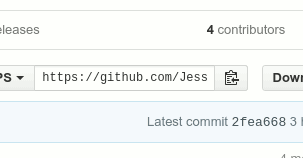
\includegraphics[width=0.9\columnwidth]{clone-url}
      \end{figure}
    \end{column}
  \end{columns}
\end{frame}

\begin{frame}[fragile=singleslide]
  \frametitle{Staging files}

  \consolefile[fontsize=\scriptsize]{src/staging.sh-session}
\end{frame}

\begin{frame}[fragile=singleslide]
  \frametitle{Committing files}

  \consolefile[fontsize=\large]{src/commit.sh-session}
\end{frame}

\begin{frame}[fragile=singleslide]
  \frametitle{Changing your mind}

  \consolefile[fontsize=\scriptsize]{src/unstage.sh-session}
\end{frame}

\begin{frame}[fragile=singleslide]
  \frametitle{Push It}

  \consolefile[fontsize=\normalsize]{src/push.sh-session}
\end{frame}

\begin{frame}[fragile=singleslide]
  \frametitle{Success!}

  \begin{figure}
    \centering
    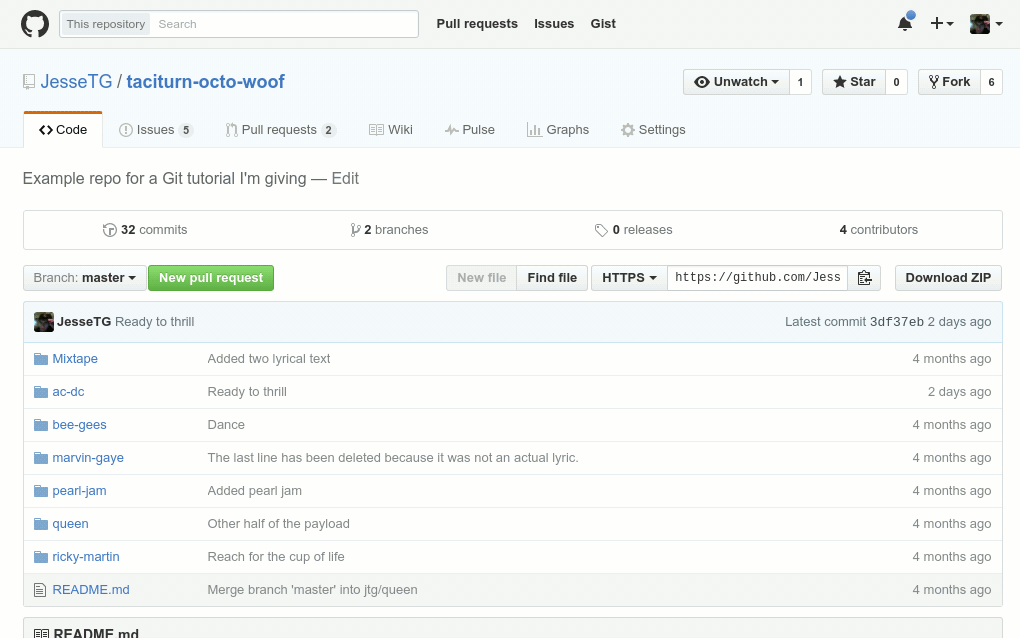
\includegraphics[width=0.9\columnwidth]{img/push-success}
  \end{figure}
\end{frame}

\begin{frame}[fragile=singleslide]
  \frametitle{What Not to Commit}

  \begin{itemize}
    \item Create a \textcolor{cyan}{.gitignore} file in your repo's root
    \item List of files/directories to not track
    \item Content varies depending on your tools and workflow
    \item \href{https://github.com/github/gitignore}{GitHub has a repo full of these}
    \begin{itemize}
      \item No, seriously, look at it
    \end{itemize}
  \end{itemize}

  \bashfile[fontsize=\small]{src/.gitignore}
\end{frame}

\begin{frame}[fragile=singleslide]
  \frametitle{What Not to Commit}

  \begin{itemize}
    \item Anything that's not human-made
    \begin{itemize}
      \item Compiled binaries, HTML docs, logs...
    \end{itemize}
    \item Large binary files
    \begin{itemize}
      \item Small ones okay if few people change them 
    \end{itemize}
    \item Sensitive information
    \begin{itemize}
      \item If you push it, \textcolor{red}{\textbf{it's compromised}}
    \end{itemize}

    \item Git repos grow, rarely shrink
    \item Excessive files are hard to merge
  \end{itemize}
\end{frame}

\begin{frame}[fragile=singleslide]
  \frametitle{Branching Code}

  \consolefile[fontsize=\small]{src/branch.sh-session}

  \begin{figure}[b]
    \centering
    \includesvg[width=0.9\columnwidth]{branch}
  \end{figure}
\end{frame}

\begin{frame}[fragile=singleslide]
  \frametitle{And again (but only partially)}

  \consolefile[fontsize=\small, escapeinside=~~]{src/interactive-patch.sh-session}
\end{frame}

\begin{frame}[fragile=singleslide]
  \frametitle{Let's push this branch}

  \consolefile[fontsize=\scriptsize]{src/another-push.sh-session}
\end{frame}

\begin{frame}[fragile=singleslide]
  \frametitle{Take a look}

  \begin{figure}
    \centering
    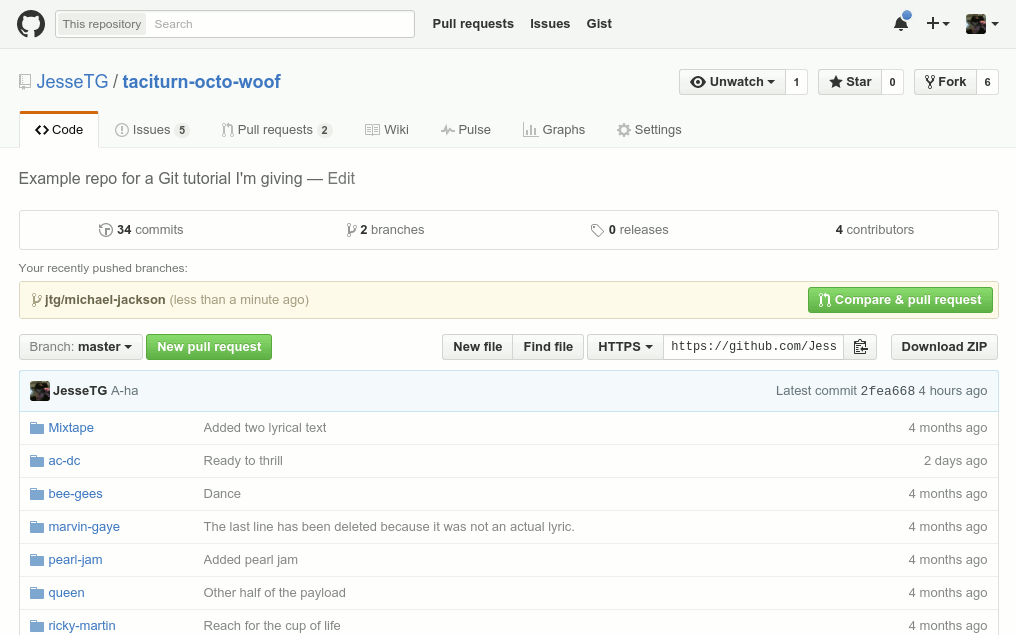
\includegraphics[width=0.9\columnwidth]{pull-request}
  \end{figure}
\end{frame}

\begin{frame}[fragile=singleslide]
  \frametitle{Make a pull request}

  \begin{figure}
    \centering
    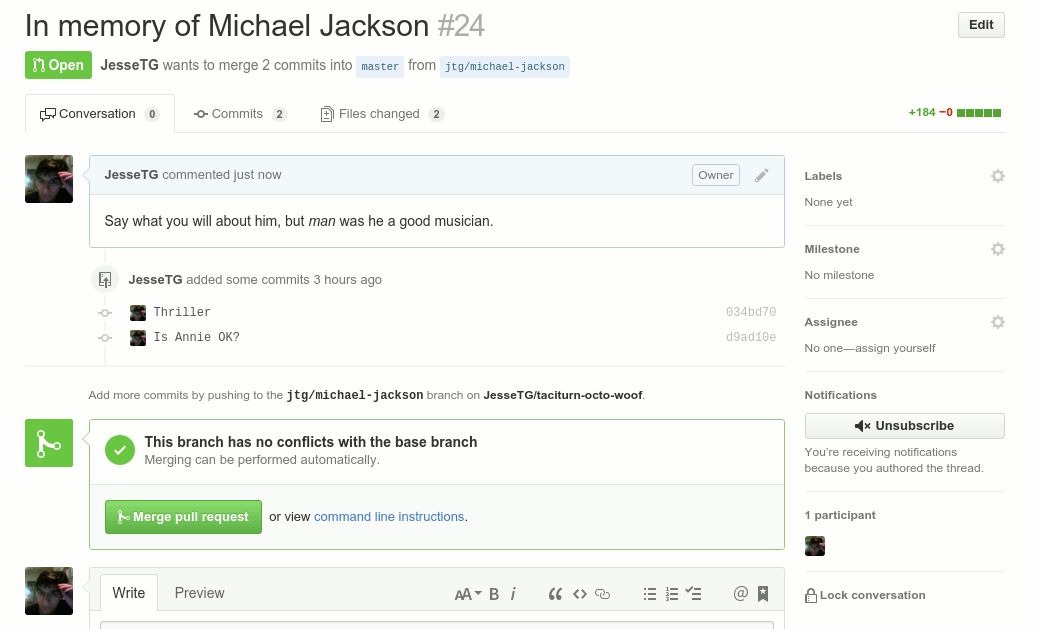
\includegraphics[width=0.9\columnwidth]{pr-pending}
  \end{figure}
\end{frame}

\begin{frame}[fragile=singleslide]
  \frametitle{Uh-oh}

  \begin{figure}
    \centering
    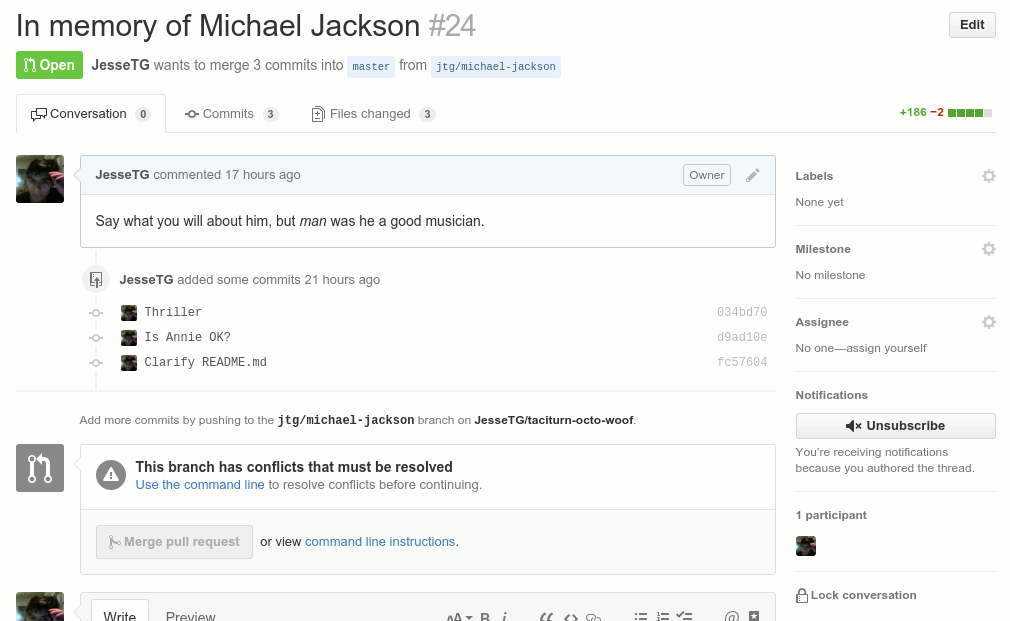
\includegraphics[width=0.9\columnwidth]{merge-conflict}
  \end{figure}
\end{frame}

\begin{frame}[fragile=singleslide]
  \frametitle{Don't panic!}

  \consolefile[fontsize=\scriptsize]{src/merge-oops.sh-session}

  \textfile[fontsize=\scriptsize, escapeinside=??]{src/merge.md}
\end{frame}


\begin{frame}[fragile=singleslide]
  \frametitle{All done!}

  \begin{figure}
    \centering
    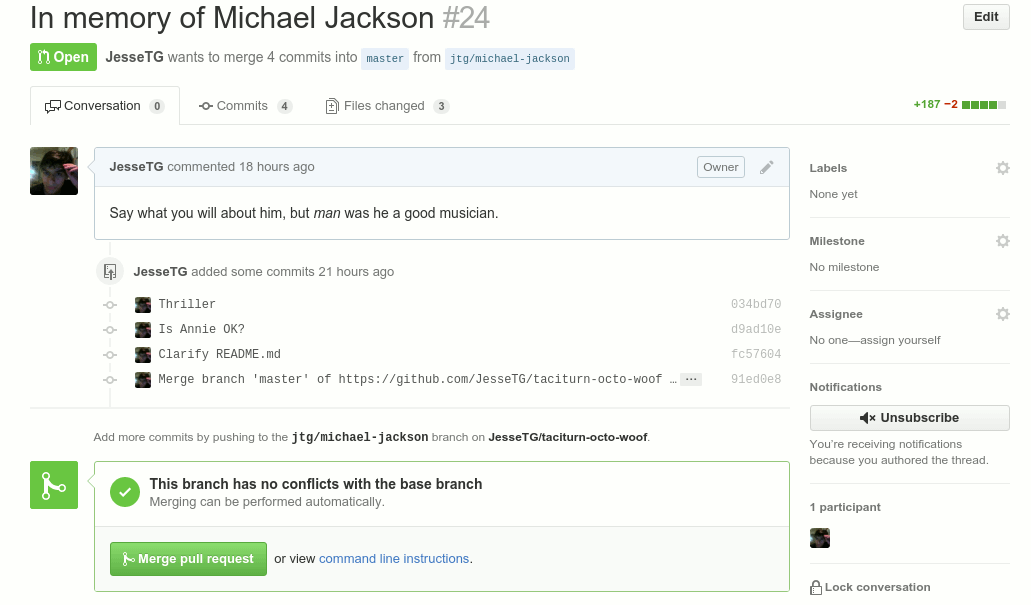
\includegraphics[width=0.9\columnwidth]{merge-resolve}
  \end{figure}
\end{frame}

\begin{frame}[fragile=singleslide]
  \frametitle{Conventions}

  \begin{itemize}
    \item \textcolor{cyan}{master:} Your repo's canonical branch
    \begin{itemize}
      \item Should always be working and mostly bug-free
      \item Never commit directly to it
      \item Changes get merged into it (and pulled from it)
    \end{itemize}
    \item \textcolor{cyan}{origin:} Your repo's canonical remote
    \begin{itemize}
      \item Usually the instance stored on GitHub
      \item Can also be your own server
    \end{itemize}
    \item \textcolor{cyan}{upstream:} Remote pointing to the repo you forked
    \item \textcolor{cyan}{<initials/branch-name>:} My branch name convention
    \item Commit messages
    \begin{itemize}
      \item All text written in imperative tense
      \begin{itemize}
        \item \enquote{I fixed that memory leak the texture loader had}  \textcolor{red}{\emph{No}}
        \item \enquote{Fix texture loader's memory leak}  \textcolor{green}{\emph{Yes}}
      \end{itemize}
      \item First line is a sentence summarizing changes
      \item Blank line
      \item Bullet points detailing the changes
    \end{itemize}
  \end{itemize}
\end{frame}

\begin{frame}[fragile=singleslide]
  \frametitle{Your turn!}

  \begin{itemize}
    \item \href{https://github.com/JesseTG/taciturn-octo-woof}{Fork this repo}
    \item Make a new branch
    \item Add at least two songs in separate files with one commit
    \begin{itemize}
      \item Can't do this with GitHub's web editor!
    \end{itemize}
    \item I'll merge a PR or three
    \begin{itemize}
      \item Or reject them, if I hate your taste in music
    \end{itemize}
  \end{itemize}
\end{frame}

\begin{frame}[fragile=singleslide]
  \frametitle{Forking other repos}

  \begin{columns}[t]
    \begin{column}{6cm}
      \begin{itemize}
        \item For contributing to open source projects
        \item Not needed when working with teammates
        \item Workflow is otherwise similar
      \end{itemize}
    \end{column}

    \begin{column}{6cm}
      \begin{figure}
        \centering
        
\includegraphics[width=0.9\columnwidth]{fork}
      \end{figure}

      \begin{figure}
        \centering
        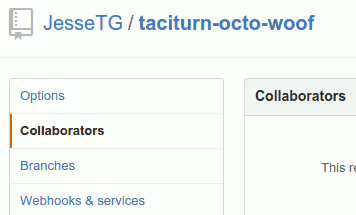
\includegraphics[width=0.9\columnwidth]{collaborators}
      \end{figure}
    \end{column}
  \end{columns}

\end{frame}

\begin{frame}[fragile=singleslide]
  \frametitle{Keeping a fork up to date}

  \consolefile[fontsize=\scriptsize]{src/sync-fork.sh-session}
\end{frame}

\begin{frame}[fragile=singleslide]
  \frametitle{Your turn!}

  \begin{itemize}
    \item Update your fork with the changes I just made.
    \item Submit another pull request, with more song lyrics.
  \end{itemize}
\end{frame}

\begin{frame}[fragile=singleslide]
  \frametitle{Issue Tracking}

  \begin{displayquote}
    If you are developing code, even on a team of one, without an organized database listing all known bugs in the code, you are going to ship low quality code. Lots of programmers think they can hold the bug list in their heads. Nonsense.
  \end{displayquote}

  \begin{flushright}
    \href{http://www.joelonsoftware.com/articles/fog0000000029.html}{-- Joel Spolsky, Fog Creek Software}
  \end{flushright}

  \begin{figure}
    \centering
    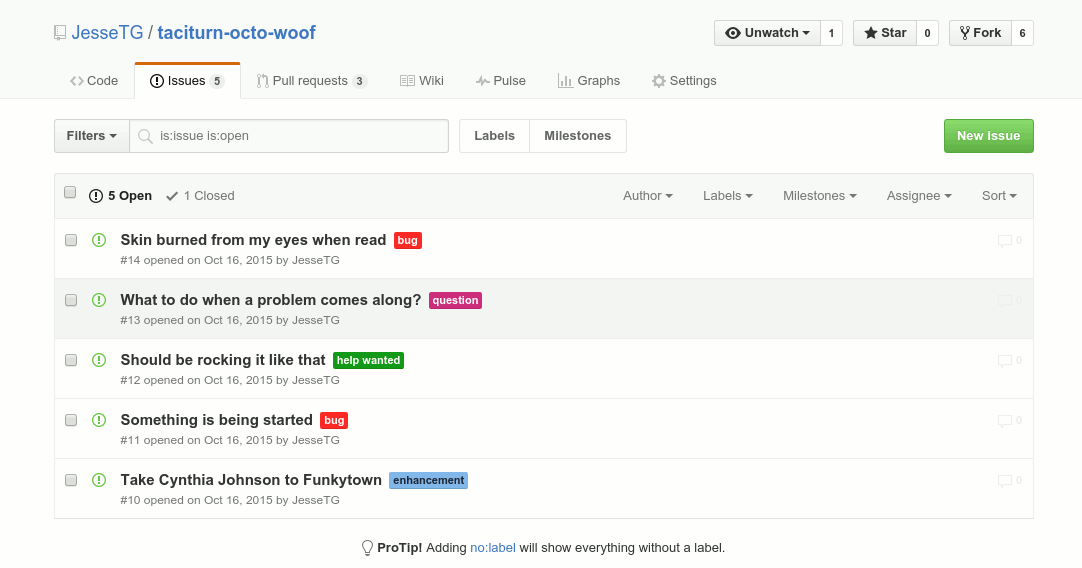
\includegraphics[width=0.75\columnwidth]{issues}
  \end{figure}
\end{frame}

\begin{frame}[fragile=singleslide]
  \frametitle{Contributing to Open Source Projects}

  \begin{itemize}
    \item You're a hobbyist
    \item You want to improve software you're using
    \item You want to be a better programmer
    \begin{itemize}
      \item Reading other people's code is just as important as writing your own!
    \end{itemize}
    \item Doesn't have to be a large project!
  \end{itemize}
\end{frame}

\begin{frame}[fragile=singleslide]
  \frametitle{Pull Request Etiquette}

  \begin{itemize}
    \item Describe your PRs thoughtfully
    \item Use the code style that already exists
    \item Add tests for new features
    \item Start small
    \item \emph{Listen to the maintainers}
    \item \textcolor{cyan}{git add --patch} (Or else you get \href{https://github.com/g-truc/glm/commit/1b9872138de05f993570062ffa30175ef843f6f7#diff-0}{this})
  \end{itemize}
\end{frame}

\begin{frame}[fragile=singleslide]
  \frametitle{Other useful Git things}

  \begin{itemize}
    \item \textcolor{cyan}{git clean -xdf:} Remove all untracked files and directories (including ignored ones)
    \item \textcolor{cyan}{git bisect:} Find out when a bug was introduced with binary search
    \item \textcolor{cyan}{git rebase -i:} Rewrite a branch's history \textcolor{red}{if it's absolutely necessary.}
    \begin{itemize}
      \item For you it won't be, but if a maintainer asks, this is what they mean
    \end{itemize}
    \item \textcolor{cyan}{git help -a:} List git's many subcommands
  \end{itemize}
\end{frame}

\begin{frame}[fragile=singleslide]
  \frametitle{Further resources}

  \begin{itemize}
    \item \textcolor{cyan}{\href{https://git-scm.com/}{Official website}:} Even has a free eBook!
    \item \textcolor{cyan}{\href{https://www.codeschool.com/}{Code School}:} Quality interactive tutorials for \$30/month
    \item \textcolor{cyan}{\href{https://www.codecademy.com/}{Codecademy}:} Recently introduced Git tutorials
    \item \textcolor{cyan}{\href{http://pcottle.github.io/learnGitBranching/}{Learn Git Branching}:} Interactive tutorial on branching
    \item \textcolor{cyan}{\href{http://devdocs.io/}{DevDocs}:} Reference for lots of tech (including Git)
    \item \textcolor{cyan}{\href{http://www.gitguys.com/}{GitGuys}:} More Git material, made intuitive
  \end{itemize}
\end{frame}

\end{document}